\section{Permutaciones}

\begin{definicion}
Dado un conjunto finito $A$ una permutación del conjunto $A$ es una ordenación de los elementos de $A$. 
\end{definicion}

De manera más explicada una permutación del conjunto $A$ es listar a todos los elementos de $A$ y darles una determinada posición, por ejemplo si $A=\{a, b ,c ,d\}$, las listas $\mathbf{abdc, dacb}$ son dos permutaciones de los elementos de $A$. 
%Diremos que una \textit{permutación} es \textbf{una ordenación de una lista de objetos}. Por ejemplo, colocar a cuatro personas en una línea equivale a encontrar permutaciones de cuatro objetos. De manera más abstracta, cada uno de los siguientes es una permutación de las letras $a$, $b$, $c$ y $d$.
%\begin{eqnarray*}
%    a,b,c,d\\
%    a,c,d,b\\
%    b,d,a,c\\
%    d,c,b,a\\
%    c,a,d,b
%\end{eqnarray*}
Se debe tener en cuenta que todos los objetos deben aparecer en una permutación y dos ordenaciones se consideran diferentes si algún objeto aparece en un lugar diferente en las ordenaciones.\\

Las permutaciones son importantes en una variedad de problemas de conteo (particularmente aquellos en los que el orden es importante), así como en otras áreas de las matemáticas.\\

El ejemplo más simple de una permutación es el caso en el que todos los objetos deben organizarse, como se hizo en la previamente para $a$, $b$, $c$, $d$. La pregunta se convierte así en la siguiente:
\begin{center}
    \textbf{Dada una lista de $n$ objetos, ¿cómo se pueden contar todas las permutaciones posibles?}
\end{center}
Sea $P_n$ el número de todas las permutaciones de un conjunto de $n$ elementos, utilizando recursividad tenemos que:
\begin{itemize}
    \item Si la lista contiene un solo elemento, entonces solo hay una permutación posible, así $P_1=1$.
    \item Si la lista contiene $n$ elementos para contar todas las permutaciones podemos separarlos en $n$ casos disjuntos. Si $A=\{a_1, a_2, \cdots a_n\}$, contar el total de permutaciones cuyo primer elemento es $a_1$ es igual a $P_{n-1}$ pues solo tenemos que saber el total de maneras de ordenar los $n-1$ elementos restantes. Así mismo contar el total de permutaciones cuyo primer elementos es $a_2$ también es $n-1$, podemos hacer este proceso para cada $n$ y luego usar el principio de la suma dado que todas las permutaciones anteriores son distintas y así obtenemos que $$P_n=\underbrace{P_{n-1}+P_{n-1}+\cdots P_{n-1}}_{\text{$n$ veces}}=nP_{n-1}$$
    
    \item Entonces tenemos 
    \begin{eqnarray*}
        P_{n} & = & n P_{n-1}\\
        & = & n(n-1)P_{n-2}\\
        & \cdots &\\
        & = & n(n-1)(n-2)\cdots 2\cdot 1 =n!
    \end{eqnarray*}
\end{itemize}

Acabamos de demostrar entonces el siguiente teorema.

\begin{teorema}
    El número de permutaciones $P_n$ de un conjuntos de cardinal $n$ es $n!$.
\end{teorema}

El teorema anterior es más común demostrarlo con el argumento siguiente que requiere el principio de la multiplicación.

Dado que cada permutación es una ordenación, comience con una ordenación vacía que consta de $n$ posiciones en una línea que se llenará con los $n$ objetos. Hay $n$ opciones para elegir qué objeto colocar en la primera posición. Después de colocar el primer objeto, quedan $n-1$ objetos, por lo que hay $n-1$ opciones para elegir qué objeto colocar en la segunda posición. Repitiendo este argumento, hay $n-2$ opciones para la tercera posición, $n-3$ opciones para la cuarta posición, y así sucesivamente. Para la $n$-ésima posición, el número de opciones es $n-(n-1)= 1$. Entonces la regla del producto implica que el total de todas las permutaciones es:
\[ P_n= n\times (n-1)\times (n-2)\times(n-3)\times \ldots \times 1=n!\]

\begin{ejemplo}
Marisol tiene cinco adornos diferentes que quiere colocar en línea sobre su escritorio. ¿De cuántas maneras puede acomodar los adornos?
\end{ejemplo}
Podemos pensar en el escritorio de Lisa como si tuviera cinco posiciones en una línea. Hay $5$ adornos, lo que da $5$ opciones para elegir qué adorno va en la primera posición. Después de colocar el primer adorno, hay 4 opciones de elegir qué adorno colocar en la segunda posición. Repitiendo este argumento, hay 3 opciones para la tercera posición, 2 opciones para la cuarta posición y 1 opción para la última posición. Por el principio de la multiplicación, el total de formas para ubicar el adorno es:
\[5\times 4\times 3\times 2\times 1=120\]


\begin{ejemplo}
Mauricio está jugando con una baraja estándar de $52$ naipes. Barajea las cartas y luego voltea la carta superior para mostrar un as de espadas. Si continúa repartiendo las cartas de la parte superior de la baraja, ¿cuántas permutaciones diferentes hay para las cartas restantes de la baraja?
\end{ejemplo}
\begin{solucion}
    Dado que la primera carta es un as de espadas, quedan $51$ cartas distintas en la baraja. Entonces hay $51!$ diferentes permutaciones de las cartas restantes.
\end{solucion}
\section{Variaciones o Arreglos}

\begin{definicion}
Un arreglo es una lista ordenada de $k$ elementos distintos de un conjunto de cardinal $n$ con $k\leq n$.
\end{definicion}

El total de arreglos de $k$ elementos de un conjunto de cardinalidad $n$ se denota por $A_n^k$ o también como $P_n^k$.

Considere el siguiente problema:

\begin{center}
    Lisa tiene $13$ adornos diferentes y quiere poner $4$ adornos en su manto. ¿De cuántas maneras es esto posible?
\end{center}
Usando la regla del producto, Lisa tiene $13$ opciones para qué adorno colocar en la primera posición, $12$ para la segunda posición, $11$ para la tercera posición y $10$ para la cuarta posición. Entonces, el número total de opciones que tiene es $13 \times 12 \times 11 \times 10$. Observar que usando la notación factorial, esto es equivalente al número total de elecciones
\[13\times 12\times 11\times 10=\frac{13\times 12\times 11\times 10\times 9!}{9!}=\frac{13!}{9!}\]

Usando el mismo argumento, podemos proceder con el caso general. \textbf{Si tenemos $n$ objetos y queremos ordenar $k$ de ellos en una fila}, hay $\displaystyle\frac{n!}{(n-k)!}$ maneras de hacer esto. Por lo tanto el total de arreglos de longitud $k$ está dado por $$A_n^k = \dfrac{n!}{(n-k)!}.$$

Como vemos la idea de arreglo está ligada a la de permutación por lo cual también es común en lugar de arreglo o variación llamar a este como una permutación de tamaño $k$ de $n$ elementos cuya notación es $P_n^k$. Los arreglos y el número combinatorio están ligados mediante la fórmula del siguiente teorema.

\begin{teorema}
    Dados un conjunto de tamaño $n$ y $k\leq n$. El total de arreglos y de combinaciones de longitud $k$ están relacionadas mediante $$A_n^k=k! \binom{n}{k}$$ 
\end{teorema}

\begin{demostracion}
    La demostración es inmediata con la fórmula del combinatorio, no obstante haremos una prueba distinta.

    Cada variación es una lista de $k$ elementos de los $n$ que hay. Dado un subconjunto de $k$ elementos de los $n$ disponibles el total de variaciones cuyos elementos son los elementos de este subconjunto es $k!$, haciendo este procedimiento para cada subconjunto de $k$ elementos luego sumando tendremos las variaciones posibles $A_n^k$. Dado que hay $\displaystyle\binom{n}{k}$ formas de seleccionar un subconjunto de tamaño $k$ y por cada subconjunto de estos hay $k!$ formas de ordenarlo, entonces por el principio de la multiplicación $$A_n^k=k! \binom{n}{k}.$$
\end{demostracion}

\begin{ejemplo}
    ¿Cuántas contraseñas de $4$ caracteres se pueden formar si los caracteres permitidos para usar sin repetición son $0, 1, 2, 3, ..., 9$ y $A, B, C, ..., Z$ y $a, b, c, ..., z$?
\end{ejemplo}
\begin{solucion}
    Utilizando el principio de la suma, tenemos que el total de caracteres a elegir viene dado por
    \[10+26+26=62\;.\]
    Así que tenemos que organizar $4$ objetos de los $62$ objetos disponibles, el número de formas de hacerlo es igual a
    \[P^{62}_4=\frac{62!}{(62-4)!}=\frac{62!}{58!}=\frac{62\times 61\times 60\times 59\times 58!}{58!}=62\times 61\times 60\times 59=13388280\]
    Por tanto, existen $13388280$ arreglos posibles.
\end{solucion}
\begin{ejemplo}
Si hay 25 aeropuertos en una línea de aviones, ¿cuántos tipos de boletos sencillos de segunda clase se deben imprimir para que un pasajero pueda viajar de una estación a otra?
\end{ejemplo}

\begin{solucion}
Es como elegir dos aeropuertos de $25$ aeropuertos. El orden de los aeropuertos (inicio y destino) es importante, es decir, $A\longrightarrow B$ no es lo mismo que $B\longrightarrow A$. Por lo tanto, usamos la permutación para seleccionar dos de $25$, es decir,
\[P^{25}_2=\frac{25!}{(25-2)!}=\frac{25!}{23!}=\frac{25\times 24\times 23!}{23!}=25\times 24=600\]
\end{solucion}
Y por lo tanto, se deben hacer $600$ boletos.
\section{Permutaciones circulares.}

Las permutaciones que se han tratado hasta ahora se llaman permutaciones lineales, como el lector podrá observar consisten en ordenar de diversas maneras una lista de elementos, imagínemos que esta lista es cerrada o más bien circular; en este caso no hay primero ni último elemento, de hecho ningún elemento tiene una posición determinada, aún así es posible configurar de diversas formas la lista dado que si importa la posición que guardan entre sí los elementos.

\begin{definicion}[Permutación circular] 

Dados $n$ elementos, una permutación circular es una configuración u ordenamiento en el que solo nos interesa la pasición relativa que guardan entre sé los elementos y no la posición que ocupan. 
\end{definicion}

Denotaremos como $C_n$ al total de permutaciones circulares de $n$ objetos. Para entender mejor el concepto, consideremos una lista de 4 elementos distintos $a, b, c$ y $d$, imaginemos que ubicamos estos en una circunferencia, como ya hemos dicho solo nos interesa la posición que guardan entre sí, por lo cual podemos pensar como si un elemento ve al centro de la circunferencia y solo le interesa saber que elemento tiene a su derecha y a su izquierda; así en la figura adjunto las configuraciones 1, 2 y 3 son permutaciones circulares distintas, mientras que configuración 4 tenemos la misma permutación circular que la configuración 1.

\begin{center}
    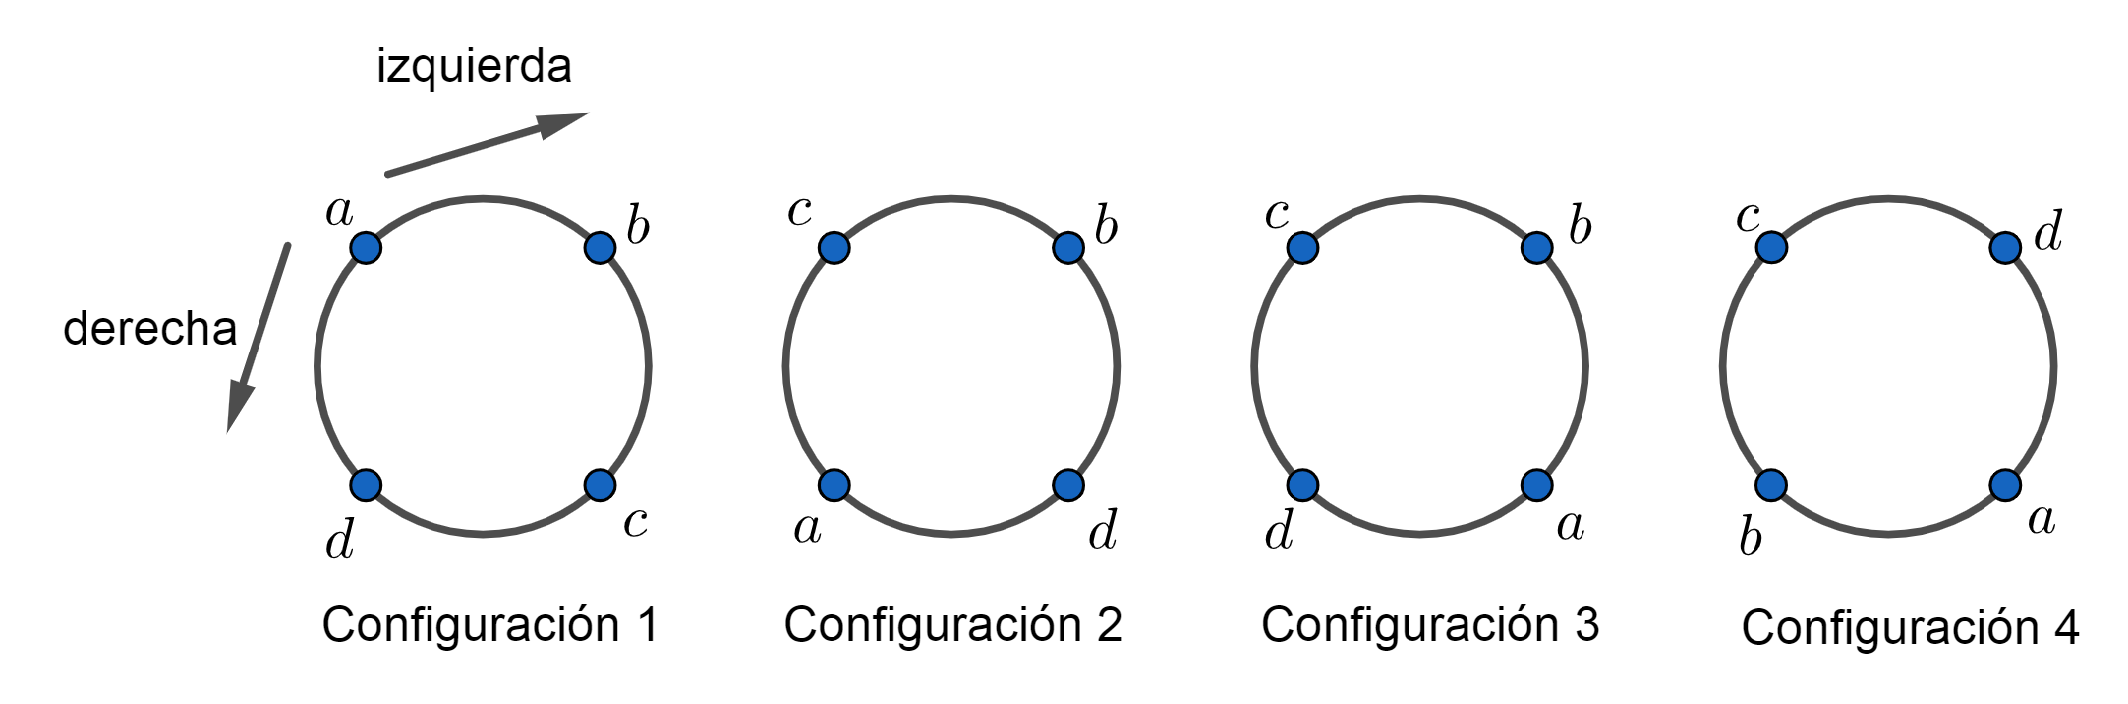
\includegraphics[scale=0.25]{Imagenes/IMG5/S1-5-01.png}
\end{center}

La configuración 1 y la configuración 3 guardan una similitud, sin embargo son permutaciones distintas, pues a pesar que en el sentido antihorario el elemento $b$ sigue después de $a$ y luego en ese orden le preceden $c$ y $d$, en la configuración 1 van en ese mismo orden pero en sentido horario. De manera más clara $a$ tiene a sus izquierda a $b$ en la configuración 1 mientras que en la configuración 3 tiene a su derecha a $b$.\\

\begin{teorema}
    El total de permutaciones circulares $C_n$ de $n$ elementos es $$C_n=\dfrac{P_n}{n}=(n-1)!.$$
\end{teorema}

\begin{demostracion}
Para ubicar a $n$ objetos en el contorno de una circunferencia pensemos primero que estos estan en una lista, luego se toma este segmento uniéndolo por sus extremos como vemos en la siguiente figura. 
\begin{center}
    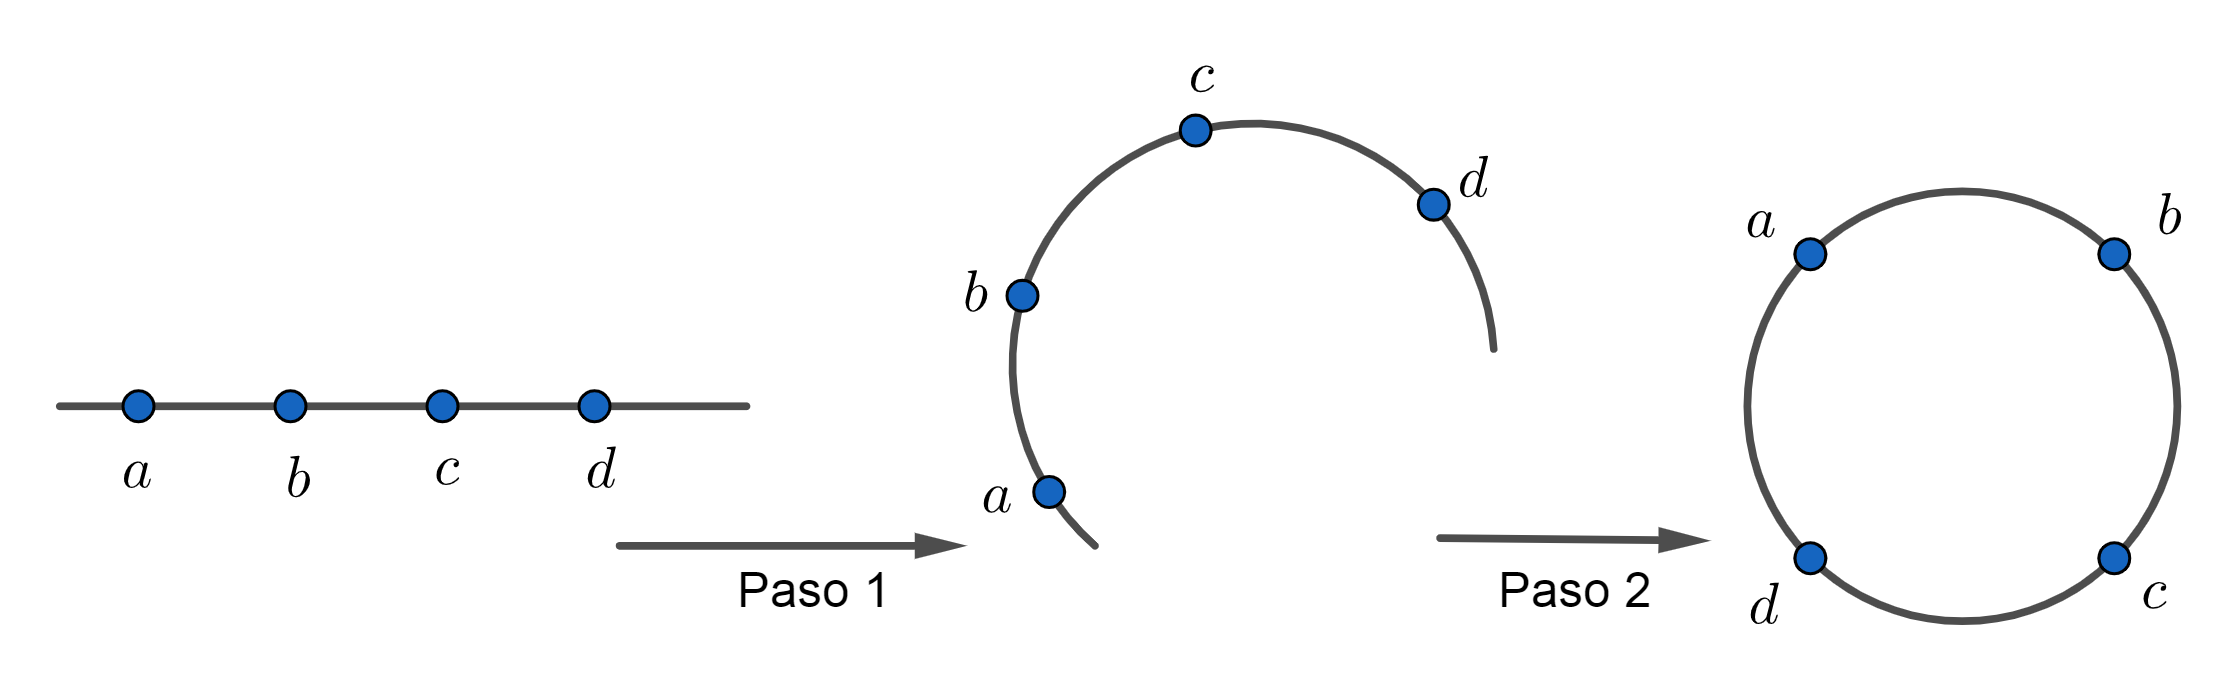
\includegraphics[scale=0.25]{Imagenes/IMG5/S1-5-02.png}
\end{center}

Notemos que los ordenamientos $abcd, dabc, cdab$ y $bcda$ luego de hacer los pasos anteriores nos darían la misma permutación circular; en efecto, pues lo común en estas permutaciones es que los elementos tienen los mismos elementos a sus derecha e izquierda al cerrar el segmento. Podemos concluir que para la permutación circular de la derecha hay 4 permutaciones lineales que darían la misma configuración. Más generalmente para cualquier permutación circular de $n$ objetos hay exactamente $n$ permutaciones lineales distintas. Como el total de permutaciones lineales es $P_n$, entonces el total de permutaciones circulares $C_n$ es $$C_n=\dfrac{P_n}{n}.$$
\end{demostracion}

\begin{ejemplo}
¿De cuántas maneras diferentes $4$ amigos se podrán ubicar alrededor de una mesa circular? 
\end{ejemplo}
\begin{solucion}
Se toma un lugar como punto de referencia, eso implica que a los otros tres lugares se les tomará como si fuese una permutación lineal. Por lo cual, tenemos
\[C_4=(4-1)!=3!=6\]
\end{solucion}

\begin{ejemplo}
    ¿De cuántas maneras distintas se pueden ubicar a $5$ parejas de esposos alrededor de una fogata, de tal manera que cada matrimonio permanezca siempre junto?
\end{ejemplo}

\begin{solucion}
Primero debemos de ordenar a cada pareja por separado y luego a todos juntos en forma circular y la idea clave es tomar a cada pareja como un sólo objeto. Ahora, cada pareja se puede ubicar de $2!$ maneras y como tenemos $5$ parejas, estas se pueden ordenar de $C_5=(5-1)!$ maneras. Por el principio de la multiplicación
\[\underbrace{2!\times 2!\times 2!\times 2!\times 2!}_{\text{por parejas}}\underbrace{\times}_{\text{y}}\underbrace{(5-1)!}_{\text{juntos}}=32\times 4!=768\]
\end{solucion}
Por tanto, hay $768$ maneras de ordenar a las parejas.


\section{Permutaciones con repetición.}
Hasta ahora hemos permutado elementos diferentes; es decir, que se pueden distinguir. Sin embargo, ese no siempre es el caso. Hay situaciones en las que entre los elementos a ordenar hay dos objetos o más que son idénticos, entonces algunas permutaciones dejarían la configuración igual. En estos casos decimos que estamos ante una permutación con repetición. El siguiente ejemplo ilustra esta situación.

\begin{ejemplo}
Supongamos que queremos hallar el total de permutaciones de la palabra \textbf{BANANA}, para fijar ideas en el proceso de hallar todas las permutaciones posibles, notemos que la letra A se repite 3 veces, si estas estuvieran etiquetadas y permutamos solo las letras A etiquetadas dejando el resto fijo tendremos $3!=6$ posibilidades como se ilustra en la figura.
\end{ejemplo}
\begin{center}
    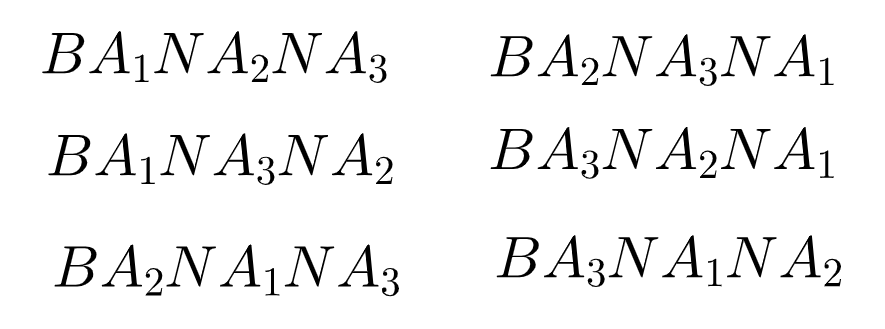
\includegraphics[scale=0.25]{Imagenes/IMG5/S1-5-03.png}
\end{center}

Si borramos el subíndice tenemos que todas las configuraciones anteriores coresponden a BANANA. Podemos saber el total de permutaciones de $n$ elementos donde alguno se repite $k$ veces a partir del total de permutaciones que hay si los elementos fueran distintos; en tal caso sabemos que hay $n!$, ahora notemos que si un elementos se repite $k$ veces por cada configuración hay $k!$ permutaciones distintas si los elementos estuviesen etiquetados, en el ejemplo podemos ver que hay 6 permutaciones distintas si las letras $A$ tendrían etiquetas; sin las etiquetas estas son la misma configuración BANANA. Pero si se repiten otros elementos entoces en $n!$ estaríamos contando la misma permutación como si los elementos fueran repetidos, si volvemos al ejemplo vemos que las letras N se repiten, entonces si las etiquetamos tendremos $3! 2!=12$ permutaciones que corresponden a la configuración BANANA.

\begin{center}
    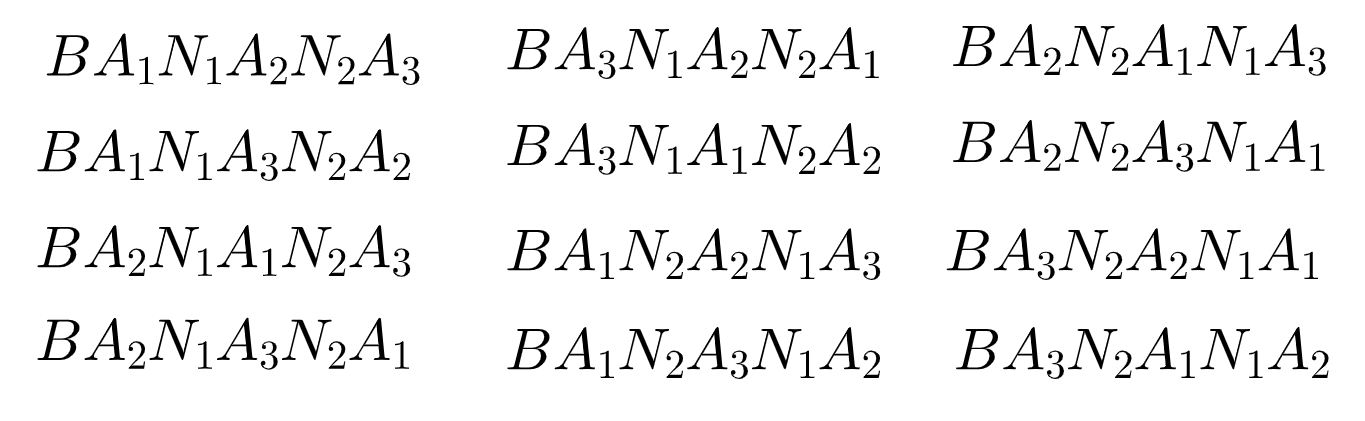
\includegraphics[scale=0.25]{Imagenes/IMG5/S1-5-04.png}
\end{center}

Generalmente tenemos que si en una lista de $n$ elementos hay $r$ elementos que se repiten $k_1, k_2\cdots k_r$ veces respectivamente con $k_i\geq 2$, entonces si pensamos como si todos los $n$ elementos fuesen distintos por cada permutación con repetición hay $k_1! k_2! \cdots k_r!$ permutaciones distintas si los elementos fueran todos distintos, por lo tanto el total de permutaciones con repetición denotado $P_{k_1, k_2, \cdots k_r}^n$ está dado por $$P_{k_1, k_2, \cdots k_r}^n=\dfrac{n!}{k_1! k_2! \cdots k_r!}.$$   

\begin{ejemplo}
Volviendo al ejemplo, el número total de permutaciones distintas que se pueden formar con las letras de la palabra \textbf{BANANA} se obtiene de la siguiente manera.  Número de palabras que se podría formar es: $6!$ 
Como ocurre la repetición $(AAA)$, debemos dividir este arreglo entre ellas dividendo el total entre 3!. Y asimismo para $(NN)$ diviendo el total entre $2!$. Por lo cual hay
\[\frac{6!}{2!\times 3!}=60\]
Y hay $60$ palabras diferentes.
\end{ejemplo}

\begin{ejemplo}
¿Cuántos números diferentes de 6 dígitos se pueden obtener usando los dígitos $5,5,7,7,7,8$?
\end{ejemplo}
\begin{solucion}
 En este caso, vemos que el número $5$ se repite $2$ veces, el número $7$ se repite $3$ veces y el número $8$ tan solo aparece una vez. Luego tenemos que
 \[P^{\;6}_{\;1;2;3}=\frac{6!}{1!\times 2!\times 3!}=60\]
 Es decir, existen un total de $60$ número para formar con los dígitos dados.
\end{solucion}
\begin{ejemplo}
¿De cuántas maneras diferentes se pueden ordenar en una fila seis sodas negras, dos rojas y cuatro amarillas?
\end{ejemplo}
\begin{solucion}
Notemos que
\begin{eqnarray*}
    n&=&6\\
    r&=&2\\
    a&=&4\\
\end{eqnarray*}
Tenemos un total de $n+r+a=6+2+4=12$ elementos. Por tanto, los arreglos a formar se calculan de la siguiente manera:
\[P^{\;12}_{\;n;r;a}=\frac{12!}{6!\times 2!\times 4!}=13860\]
\end{solucion}

Ahora estamos listos para probar la fórmula que usamos en las primeras sesiones para el número combinatorio.

\begin{teorema}
    Dado un conjunto $A$ de cardinal $n$ el total de subconjuntos de $A$ de tamaño $k$ es $$\binom{n}{k}=\dfrac{n!}{(n-k)!k!}.$$
\end{teorema}

\begin{demostracion}
    Contar el total de subconjuntos de $k$ elementos equivale a contar el total de permutaciones de $n$ elementos donde solo hay dos elementos distinguibles y uno se repite $k$ veces, mientreas que el otro se repite $n-k$ veces; pues en algún subconjunto de $k$ elementos no importa el orden, por lo tanto se puede tratar como si todos estos elementos fueran idénticos, lo mismo sucede con el subconjunto de $n-k$ elementos, por lo tanto  $$\binom{n}{k}=\dfrac{n!}{(n-k)!k!}.$$
\end{demostracion}

\section{Problemas.}

\begin{problema}
Se desea formar un comité con un presidente, dos secretarios y tres tesoreros, para lo cuál
se dispone de 32 postulantes que pueden desempeñar cualquiera de los cargos. ¿De cuántas
maneras distintas puede quedar formado el comité?
\end{problema}

\begin{problema}
$n$ hombres ($n>2$) se encuentran sentados a una mesa redonda. Convengamos en considerar coincidentes dos disposiciones respecto a los sitios, siempre que cada hombre tengan los mismos, siempre que cada hombre tenga los mismos vecinos en ambos casos. ¿Cuántos son los modos de sentarse a la mesa?
\end{problema}

\begin{problema}
¿Cuántas permutaciones se pueden hacer con las letras de la plabra \textbf{MISSISSIPPI}? ¿Cuántas de éstas no contienen dos o más letras \textbf{I} consecutivas?
\end{problema}

\begin{problema}
Se tienen 12 personas y dos ruedas de asientos, cada una de seis lugares, una dentro de la otra, tal como se muestra en la siguiente figura. ¿De cuántas formas distintas pueden ubicarse las doce personas en los doce asientos?

\begin{figure}[h]
    \centering
    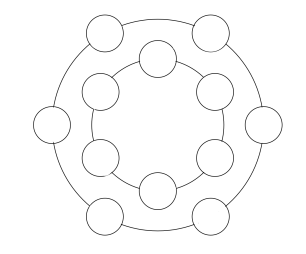
\includegraphics[scale=0.5]{Imagenes/Screenshot from 2023-12-07 15-25-24.png}
    %\caption{Caption}
    %\label{fig:enter-label}
\end{figure}

\end{problema}

\begin{problema}
¿Mediante cuántos métodos pueden sentarse a una mesa redonda $n$ hombres y $n$ mujeres de tal modo que de cada dos personas de un mismo sexo ninguna esté sentada al lado de la otra?
\end{problema}

\begin{problema}
Cada una de las diagonales y lados de un polígono regular de n lados se colorean de azul o
de rojo. ¿De cuántas formas puede hacerse la coloración?
\end{problema}

\begin{problema}
¿Cuántos números de dos mil catorce dígitos cumplen que el producto de todos sus dígitos es par?
\end{problema}

\begin{problema}
Seis matrimonios se reúnen a cenar en una mesa circular. ¿De cuántas formas pueden ubicarse,
si cada hombre debe estar entre dos mujeres y los miembros de cada pareja deben estar juntos?
\end{problema}

\begin{problema}
Se desea formar un comité con un presidente, dos secretarios y tres tesoreros, para lo cuál
se dispone de 32 postulantes que pueden desempeñar cualquiera de los cargos. ¿De cuántas
maneras distintas puede quedar formado el comité?
\end{problema}

\begin{problema}
Los dígitos $1$, $7$, y $8$ y $5$ copias del dígito $5$ están dispuestos para formar un número entero de $8$ dígitos. ¿Cuántos enteros diferentes se pueden formar?
\end{problema}

\begin{problema}
Si tenemos que 
\[P^n_2=20\cdot P^n_3\]
¿cuál es el valor de $n$?
\end{problema}
\begin{problema}
Se preparan tres banderas de color amarillo, rojo y azul para el envío de señales. Cada señal consta de una, dos o tres banderas donde se permite la repetición en el color de la bandera. Por ejemplo, \textbf{rojo, amarillo} y \textbf{azul, azul, rojo} son dos señales posibles. ¿Cuántas señales distintas se pueden hacer?
\end{problema}

\begin{problema}
    ¿De cuántas maneras se pueden sentar tres perros y dos gatos alrededor de una mesa circular? Considere que dos animales del mismo tipo son idénticos, y las configuraciones que se pueden rotar para que coincidan también se consideran idénticas.
\end{problema}

\begin{problema}
¿Cuántos números diferentes de $10$ cifras se pueden escribir usando las cifras $1$, $2$ y $3$ con la condición de que la cifra $3$ se utilice en cada número exactamente dos veces y que además est número sea divisible por $9$?
\end{problema}